% main.tex for MA2003 Complex Analysis I

%\PassOptionsToPackage{blanks}{camnotes}
\RequirePackage[demo]{graphicx}

% document class
\documentclass[oneside, 11pt]{article}

\usepackage{amsthm}
\usepackage[cm]{fullpage}

\usepackage{camnotes}

%\setscaleimages{3}
\solutioncolour{blue}
\proofcolour{blue}

% module info
%\modulecode{MA2003}
%\moduletitle{Complex Analysis I}
%\academicyear{2017-18}

%\renewcommand{\thetheorem}{\arabic{chapter}.\arabic{theorem}}
% load packages
\usepackage{amsmath}
\usepackage{comment}
\usepackage{verbatim}
\usepackage{mathtools}
\usepackage{amsfonts}
\usepackage{amssymb}
\usepackage{wrapfig}
\usepackage{setspace}

\usepackage{framed}
\usepackage{enumitem}
\usepackage{array}
\usepackage{xcolor}
\usepackage{float}
\usepackage[mode=buildnew]{standalone}% requires -shell-escape
\usepackage{sidecap}
\usepackage{version}
\usepackage{todonotes}
\sidecaptionvpos{figure}{r}
\renewcommand\sidecaptionsep{2cm}

\setstretchfactor{3} 
\setimagestretchfactor{1}

% document info
\title{Exercise Sheet 0}
\author{D McConnell}
\date{Summer 2017}

\graphicspath{{./images/}}

% new commands
\newcommand{\contint}{\int_{\mathcal{C}}}
\newcommand{\conj}[1]{\overline{#1}}
\newcommand{\conjugate}[1]{\overline{#1}}
\renewcommand{\Re}{\textsf{Re}}
\renewcommand{\Im}{\textsf{Im}}
\newcommand{\abs}[1]{\left| #1 \right|}
\newcommand{\set}[1]{\left\{#1\right\}}
\newcommand{\brac}[1]{\left( #1 \right) }
\newcommand{\pd}[2]{\dfrac{\partial #1}{\partial #2}}
\newcommand{\rlim}[2]{\lim_{\substack{#1, \\ #2}}}
\newcommand{\reverse}[1]{\widetilde{#1}}
\newcommand{\id}{\textsf{id}}
\newcommand{\Res}{\mathrm{Res}}
\newcommand{\Arg}{\mathrm{Arg}}
\newcommand{\polar}[2]{#1 \left( \cos \left( #2 \right) + i \sin \left( #2 \right) \right)}
\newcommand{\expform}[2]{ #1 \exp \left( #2 \right)}
\newcommand{\R}{\mathbb{R}}
\newcommand{\C}{\mathbb{C}}
\newcommand{\cont}{\mathcal{C}}

\DeclareMathOperator{\Log}{Log}

\let\remark\blankbox
\let\endremark\endblankbox

\newcommand{\leftimage}[2]{
\begin{tabular}{c@{\hskip 1cm} m{0.5\textwidth} }
\begin{minipage}{0.5\textwidth}
\begin{center}
\begingroup
#1
\endgroup
\end{center}
\end{minipage}
&
\blankson\begingroup
#2
\endgroup\blanksoff
\end{tabular}
}




\begin{document}
\begin{center}
{\large \bf Complex Analysis \\ Revision Exercises}

In this module it is important that you be able to work with complex numbers without difficulty.  The problems on this exercise sheet cover algebraic manipulation and basic properties of complex numbers: this material should be familiar to you already from Foundations last year.  Solutions, and the relevant lecture notes from Foundations I, are available on Learning Central.
\end{center}

% !TEX root = exercises.tex

\exercisetitle{Exercise Sheet 0}

\begin{questions}
\question Write the following complex numbers in polar form $z=r \left( \cos ( \theta)+ i \sin (\theta) \right)$ (or equivalently, $z=r \exp \left(i \theta \right)$):
\begin{parts}
\part $1+i$
\part $-1+i$
\part $1+i \sqrt{3}$
\part $\dfrac{(1+i)^7}{(1+i\sqrt{3})^2}$
\end{parts}

\begin{answer}
\begin{enumerate}
\item[(a)] $1+i=\sqrt{2} \left( \cos ( \frac{\pi}{4} ) + i \sin ( \frac{\pi}{4} ) \right)$
\item[(b)] $-1+i=\sqrt{2} \left( \cos ( \frac{3\pi}{4} ) + i \sin ( \frac{3\pi}{4} ) \right)$
\item[(c)] $1+i\sqrt{3}=2 \left( \cos ( \frac{\pi}{3} ) + i \sin ( \frac{\pi}{3} ) \right)$
\item[(d)] While we could expand the numerator and denominator and then simplify, it is much easier to use De Moivre's Theorem:
\[
r \left( \cos ( \theta) + i \sin (\theta ) \right)^n = r^n \left( \cos ( n\theta) + i \sin ( n \theta ) \right) \quad (n \in \mathbb{Z}).
\]
\begin{align*}
(1+i)^7 & = \polar{2^{7/2}}{7 \pi / 4},\\ 
(1+ i \sqrt{3})^{-2} & = \polar{2^{-2}}{-2\pi/3}.
\end{align*}
Then we get
\begin{align*}
\frac{(1+i)^7}{(1+i\sqrt{3})^2} & = (1+i)^7(1+i \sqrt{3})^{-2} \\
& = \polar{2^{3/2}}{13\pi/12}. 
\end{align*}
This is fine, however, if we wish to use the principal value of the argument, we must subtract an appropriate integer multiple of $2\pi$ from $13\pi/12$ (to ensure that the argument lies in $(-\pi,\pi]$).  This is given by  $13\pi /12-2\pi = -11\pi/12$, thus
\[
\frac{(1+i)^7}{(1+i\sqrt{3})^2} = \polar{2^{3/2}}{-11\pi /12}.
\]
An equally valid way of answering this is using the exponential polar form:
\[
(1+i)^7 = \expform{2^{7/2}}{7 \pi / 4}\qquad(1+ i \sqrt{3})^{-2} = \expform{2^{-2}}{-2\pi/3}.
\]
The properties $\exp(z_1)\exp(z_2)=\exp(z_1+z_2)$ and $\exp(z+2\pi i)=\exp(z)$  give:
\[
\frac{(1+i)^7}{(1+i\sqrt{3})^2} = \expform{2^{7/2}}{7 \pi/4} \expform{2^{-2}}{-2\pi/3}  =  \expform{2^{3/2}}{-11\pi/12}.
\]
\end{enumerate}
\end{answer}

\question 
\begin{parts}
\part For $z=a+ib$, express $z^{-1}$ (i.e, $\dfrac{1}{z}$) in Cartesian form
\part Write down the modulus and Principal Argument of $z^{-1}$ in terms of $\abs{z}$ and $\Arg (z)$.
\end{parts}

\begin{answer}
\begin{enumerate}
\item[(a)] We use the fact that $\displaystyle \frac{1}{z} = \frac{1}{z} \cdot \frac{\conj{z}}{\conj{z}} = \frac{\conj{z}}{\abs{z}^2}$ to invert any nonzero complex number:
\[
\frac{1}{a+ib} = \frac{1}{a+ib} \cdot \frac{a-ib}{a-ib} = \frac{a-ib}{a^2+b^2} = \frac{a}{a^2+b^2} - i\frac{b}{a^2+b^2}.
\]
\item[(b)] Writing $z=\polar{r}{\theta}$, De Moivre's Theorem gives
\[
z^{-1} = \left(\polar{r}{\theta}\right)^{-1} = \polar{\frac{1}{r}}{-\theta}.
\]
Hence $\abs{z^{-1}} = 1/\abs{z}$ and $\Arg (z^{-1})=-\Arg (z)$.
\end{enumerate}
\end{answer}

\question Express the following complex numbers in Cartesian form (that is to say, as $a+ib$ for $a,b \in \R$)
\[
\frac{i-1}{1-i}\qquad \frac{1}{1+i}\qquad \frac{3+4i}{1-2i}.
\]
\begin{answer}
In each case, we make the denominator of the quotient $\frac{z_1}{z_2}$ real by multiplying by $\conj{z_2}/ \conj{z_2}$, which gives
\[
\frac{z_1}{z_2} = \frac{z_1\conj{z_2}}{\abs{z_2}^2}.
\]
Thus for example
\begin{align*}
\frac{i-1}{1-i} & = \frac{i-1}{1-i} \cdot \frac{1+i}{1+i} \\
& = \frac{1}{2} \left[ i(1+i)-1(1+i) \right] \\
& = \frac{1}{2} \left[-2 \right] \\
& = -1\ (+i0).
\end{align*}
Similarly
\begin{align*}
\frac{1}{1+i} &=  \frac{1}{2} - \frac{i}{2} \\
\frac{3+4i}{1-2i} &= -1+2i.
\end{align*}
\end{answer}

\question Find the principal argument of the four points $\pm 1\pm i\sqrt{3}$.
\begin{answer}
\begin{align*}
\Arg (1+i\sqrt{3}) &= \frac{\pi}{3} \\
\Arg (-1+i \sqrt{3} ) &= \frac{2\pi}{3} \\
\Arg (-1-i\sqrt{3} ) &= - \frac{2\pi}{3} \\
\Arg (1-i\sqrt{3} ) &= - \frac{\pi}{3}. 
\end{align*}
\end{answer}




\question Calculate
\[
\Arg \left. \left( \frac{1}{2} + \frac{1}{z^2} \right) \right|_{z=1+i}.
\]
(The notation
$
\left. f(z) \right|_{z=w}
$
means $f(z)$ evaluated at $z=w$, or in other words, $f(w)$.)
\begin{answer}
We have
\[
\frac{1}{2} + \frac{1}{(1+i)^2} = \frac{1}{2}-\frac{i}{2},
\]
with principal argument $-\frac{\pi}{4}$.
\end{answer}
\question Show that
\[
2 \left( \frac{z}{z+i} \right) \left. \frac{(z+i-z)}{(z+i)^2} \right|_{z=i} = \frac{-i}{4}.
\]
\begin{answer}
\begin{align*}
2 \left( \frac{z}{z+i} \right) \left. \frac{(z+i-z)}{(z+i)^2} \right|_{z=i} & = 2 \left( \frac{i}{2i} \right) \left( \frac{i+i-i}{(2i)^2} \right) \\
& = \frac{2i}{2i} \frac{i}{(-4)} = -\frac{i}{4}.
\end{align*}
\end{answer}


\question Sketch the following regions of $\C$:
\begin{parts}
\part $1 < |z| < 2$ (This notation is shorthand for the set $\set{ z \in \C: 1 < \abs{z} <2}$.)
\part $1<|z+2|<2$
\part $1 < \Im (z-i) < 2$
\end{parts}
\begin{answer}

\begin{enumerate}
\item[(a),(b)] Note that for $\alpha \in \C$ and $r>0$, the set $\set{ z \in \C: \abs{z-\alpha} = r}$ is precisely the circle of radius $r$ centred at $\alpha$.  The sets $0<\abs{z-\alpha}<r$ and $\abs{z-\alpha}>r$ respectively are the regions inside and outside the circle.

Hence $1<z<2$ is the region outside the circle of radius 1 centred at 0, and inside the circle of radius 2 centred at 0.  The set $1<\abs{z+2}<2$ is the same but with circles centred at $-2$.  A set of this type is called an \emph{annulus}.
\begin{center}
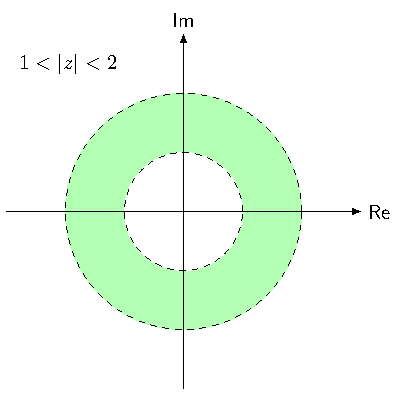
\includegraphics[scale=0.75]{annulus}\quad 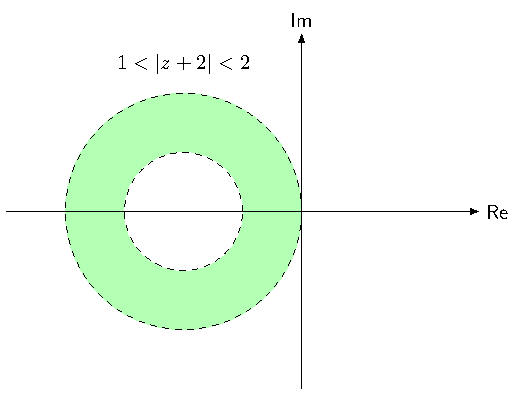
\includegraphics[scale=0.75]{annulus2}
\end{center}

\item[(c)] Write $z=x+iy$, then $z-i = x+i(y-1)$ and so
\begin{align*}
\set{z\in \C: 1 < \Im(z-i) <2 } &= \set{ x+iy \in \C : 1<y-1 <2 } \\
&= \set{x+iy \in \C: 2<y<3},
\end{align*}
which is the infinite horizontal band bounded by the lines $y=2$ and $y=3$.
\begin{center}
\oldincludegraphics[scale=0.75]{band}
\end{center}
\end{enumerate}
\end{answer}
\question 
\begin{parts}
\part Prove that for two nonzero complex numbers $z_1$ and $z_2$ we have
\[
\abs{z_1z_2} = \abs{z_1} \cdot \abs{z_2} \quad\text{ and }\quad \arg(z_1z_2)=\arg(z_1)\arg(z_2)
\]
(hint: write $z_1$ and $z_2$ in polar form).  Is it always true that $\Arg(z_1z_2)=\Arg(z_2)+\Arg(z_2)$?
\begin{answer}
Writing
\[
z_1=\polar{r_1}{\theta_1}\quad\text{and}\quad z_2=\polar{r_2}{\theta_2}
\]
we see that
\begin{align*}
z_1z_2&=r_1r_2 \left( \cos(\theta_1)\cos(\theta_2)-\sin(\theta_1)\sin(\theta_2) +i \left[ \cos(\theta_1)\sin(\theta_2)+\cos(\theta_2)\sin(\theta_1) \right] \right) \\
& = r_1r_2 \left( \cos(\theta_1+\theta_2)+i \sin(\theta_1+\theta_2) \right).
\end{align*}
Thus
\[
\abs{z_1z_2}=r_1r_2=\abs{z_1}\cdot \abs{z_2}\quad\text{and}\quad \arg(z_1z_2)=\theta_1+\theta_2=\arg(z_1)+\arg(z_2).
\]
It is not always true that $\Arg(z_1z_2)=\Arg(z_1)+\Arg(z_2)$.  Indeed, if $z_1=z_2=-1$ we have $\Arg (-1)=\pi$ but
\[
\Arg ((-1)(-1)) = \Arg (1) = 0.
\]
\end{answer}
\part Show that $\exp(z_1)\exp(z_2) = \exp(z_1+z_2)$.
\begin{answer}
With $z_1=x_1+iy_1$ and $z_2=x_2+iy_2$ a similar calculation to part (a) shows that
\begin{align*}
\exp(z_1)\exp(z_2) &= \polar{e^{x_1}}{y_1} \polar{e^{x_2}}{y_2} \\
 & = \polar{e^{x_1}e^{x_2}}{y_1+y_2} \\
 & = \polar{e^{x_1+x_2}}{y_1+y_2} = \exp(z_1+z_2).
\end{align*}
\end{answer}
\end{parts}
\question Write down the $3^{rd}$ roots of $-8$ in Cartesian form.
\begin{answer}
Writing $-8=\polar{8}{\pi}$, the three cubic roots are of the form $\polar{\sqrt[3]{8}}{(\pi+2k\pi)/3}$ for $k=0,1,2$.  In polar form, these are
\[
\polar{2}{\pi/3}, \quad \polar{2}{\pi} \quad\text{and}\quad\polar{2}{5\pi/3},
\]
or in Cartesian form $1+\sqrt{3},\ -2$ and $1-\sqrt{3}$ respectively.

\end{answer}

\question Find the values of $z$ for which $z^2+4iz-1=0$.  Which of these values lies inside the circle $C=\set{z \in \C: \abs{z}=1}$.
\begin{answer}
This is simply the usual quadratic formula: the roots of this polynomial are given by
\[
\frac{-4i\pm \sqrt{(4i)^2-4(1)(-1)}}{2} = \frac{-4i\pm i \sqrt{12}}{2} = i (-2 \pm  \sqrt{3}).
\]
To see which of these lies inside the circle $\abs{z}=1$, we examine the modulus and see that $\abs{i(-2 + \sqrt{3})} \approx 0.071<1$ and $\abs{i(-2-\sqrt{3})} \approx 1.93>1$. Thus only $i(-2+\sqrt{3})$ lies inside this circle.
\end{answer}


\question Show that $\Re (z) \leq \abs{ \Re (z)} \leq \abs{z}$ and $\abs{\Re (z)}+\abs{\Im (z)} \leq \sqrt{2} \abs{z}$.
\begin{answer}
The fact that $\Re (z) \leq \abs{ \Re (z)}$ is trivial.  Moreover,  writing $z=x+iy$ we see that
\[
\abs{\Re(z)} = \sqrt{x^2} \leq \sqrt{x^2+y^2}
\]
since $x^2 \leq x^2+y^2$ (and the square root function is increasing).

For the second inequality, note that with $z=x+iy$,
\begin{align*}
\left( \abs{\Re (z)}+\abs{\Im (z)} \right)^2 & = \left( \abs{x}+\abs{y} \right)^2 \\
& \leq \left( \abs{x}+\abs{y} \right)^2  + \overbrace{\left( \abs{x}-\abs{y} \right)^2}^{\geq 0}  \\
& = x^2+y^2+2\abs{xy} + x^2 + y^2 - 2\abs{xy} \\
& = 2(x^2+y^2) = 2 \abs{z}^2.
\end{align*}
Taking square roots of both sides yields the required inequality.
\end{answer}
\end{questions}




\end{document}